\documentclass[12pt]{article}
\usepackage[papersize={8cm,14cm},margin={.5cm,.5cm}]{geometry}
\usepackage{common}
\usepackage{amssymb}
\newcommand{\slantparallel}{\mathrel{\mkern-2mu/\mkern-4mu/\mkern-2mu}}
\begin{document}
\begin{problem}
\item[4.] 菱形 $ABCD$ 中,$E$ 點在 $\overline{BC}$ 上,$F$ 點在 $\overline{CD}$ 上,$G$ 點、$H$ 點在 $\overline{AD}$ 上,且 $\overline{AE} \slantparallel \overline{HC} \slantparallel \overline{GF}$,如圖(四)所示。若 $\overline{AH} = 8$,$\overline{HG} = 5$,$\overline{GD} = 4$,則下列何者的長度最長?
  \begin{figure}[ht]
    \centering
    \vspace*{-1ex}
    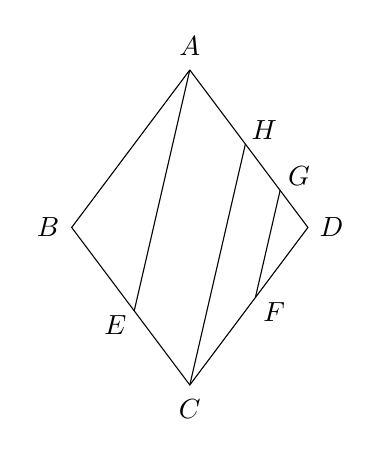
\begin{tikzpicture}
      \draw (0,2) -- (-1.5,0) -- (0,-2) -- (1.5,0) -- (0,2);
      \draw (0,2) -- (-.706,-1.059);
      \draw (.706,1.059) -- (0,-2);
      \draw (1.147,.471) -- (.833,-.889);
      \node at (0,2.3) {$A$};
      \node at (-1.8,0) {$B$};
      \node at (0,-2.3) {$C$};
      \node at (1.8,0) {$D$};
      \node at (-.946,-1.239) {$E$};
      \node at (1.073,-1.069) {$F$};
      \node at (1.387,.651) {$G$};
      \node at (.946,1.239) {$H$};
    \end{tikzpicture}
    \vspace*{-1ex}
    \caption*{圖(四)}
    \vspace*{-2ex}
  \end{figure}
  \begin{choices}
    \item $\overline{BE}$
    \item $\overline{EC}$
    \item $\overline{CF}$
    \item $\overline{FD}$
  \end{choices}
\end{problem}
\end{document}
